%\documentclass[mathserif]{beamer}
\documentclass[handout]{beamer}
%\usetheme{Goettingen}
\usetheme{Warsaw}
%\usetheme{Singapore}
%\usetheme{Frankfurt}
%\usetheme{Copenhagen}
%\usetheme{Szeged}
%\usetheme{Montpellier}
%\usetheme{CambridgeUS}
%\usecolortheme{}
%\setbeamercovered{transparent}
\usepackage[english, activeacute]{babel}
\usepackage[utf8]{inputenc}
\usepackage{amsmath, amssymb}
\usepackage{dsfont}
\usepackage{graphics}
\usepackage{cases}
\usepackage{graphicx}
\usepackage{pgf}
\usepackage{epsfig}
\usepackage{amssymb}
\usepackage{multirow}	
\usepackage{amstext}
\usepackage[ruled,vlined,lined]{algorithm2e}
\usepackage{amsmath}
\usepackage{epic}
\usepackage{epsfig}
\usepackage{fontenc}
\usepackage{framed,color}
\usepackage{palatino, url, multicol}
\usepackage{listings}
%\algsetup{indent=2em}
\newcommand{\factorial}{\ensuremath{\mbox{\sc Factorial}}}
\newcommand{\BIGOP}[1]{\mathop{\mathchoice%
{\raise-0.22em\hbox{\huge $#1$}}%
{\raise-0.05em\hbox{\L
\usepackage{fontenc}
\usepackage{framed,color}
\usepackage{palatino, url, multicol}
\usepackage{listings}
%\algsetup{indent=2em}
\newcommand{\factorial}{\ensuremath{\mbox{\sc Factorial}}}
\newcommand{\BIGOP}[1]{\mathop{\mathchoice%
{\raise-0.22em\hbox{\huge $#1$}}%
{\raise-0.05em\hbox{\Large $#1$}}{\hbox{\large $#1$}}{#1}}}
\newcommand{\bigtimes}{\BIGOP{\times}}
\vspace{-0.5cm}
\title{Introduction to Statistical Inference}
\vspace{-0.5cm}
\author[Felipe Bravo Márquez]{\footnotesize
%\author{\footnotesize  
 \textcolor[rgb]{0.00,0.00,1.00}{Felipe José Bravo Márquez}} 
\date{ \today }
arge $#1$}}{\hbox{\large $#1$}}{#1}}}
\newcommand{\bigtimes}{\BIGOP{\times}}
\vspace{-0.5cm}
\title{Linear Regression}
\vspace{-0.5cm}
\author[Felipe Bravo Márquez]{\footnotesize
%\author{\footnotesize  
 \textcolor[rgb]{0.00,0.00,1.00}{Felipe José Bravo Márquez}} 
\date{ \today }


\begin{document}
\begin{frame}
\titlepage


\end{frame}


%%%%%%%%%%%%%%%%%%%%%%%%%%%



\begin{frame}{Introduction}
\scriptsize{
\begin{itemize}

 \item  A regression model is used to model the relationship of a numerical dependent variable $\mathbf{y}$ with $n$ independent variables  $\mathbf{x}_1, \mathbf{x}_2, \dots, \mathbf{x}_n$ \cite{wasserman2013all}. 
 
 \item The dependent variable $\mathbf{y}$ is also called \textbf{target}, \textbf{outcome}, or \textbf{response} variable.
 
 \item The independent variables  $\mathbf{x}_1, \mathbf{x}_2, \dots, \mathbf{x}_n$ are also called \textbf{covariates}, \textbf{attributes}, \textbf{features}, por \textbf{predictor variables}.
 
 
 \item  Roughly speaking we want to know the expected value of $\mathbf{y}$ from the values of $\mathbf{x}$:
 \begin{displaymath}
 \mathbb{E}(y|x_1,x_2,\dots,x_n)
 \end{displaymath}

 
 \item  We use these models when we believe that the response variable $\mathbf{y}$ can be modeled by other independent variables.
 
 \item To perform this type of analysis we need a dataset consisting of $m$ observations that include both the response variable and each of the attributes.
 
 \item We refer to the process of \textbf{fitting} a regression function as the process in which from the data we infer a hypothesis function $h$ that allows us to \textbf{predict} unknown $\mathbf{y}$ values using the values of the attributes.

 
\end{itemize}



} 
 
\end{frame}


\begin{frame}{Introduction (2)}
\scriptsize{
\begin{itemize}
 
 \item This process of fitting a function from data is referred to in the areas of data mining and machine learning as \textbf{training}.

 \item In those disciplines, functions are said to \textbf{learn} from data.
 
 \item Since we need observations where the value of $\mathbf{y}$ is known to learn the function, such techniques are referred to as \textbf{supervised learning} techniques.
 
 \item When $\mathbf{y}$ is a categorical variable we have a \textbf{classification} problem.
 

 
\end{itemize}


\begin{figure}[h!]
	\centering
	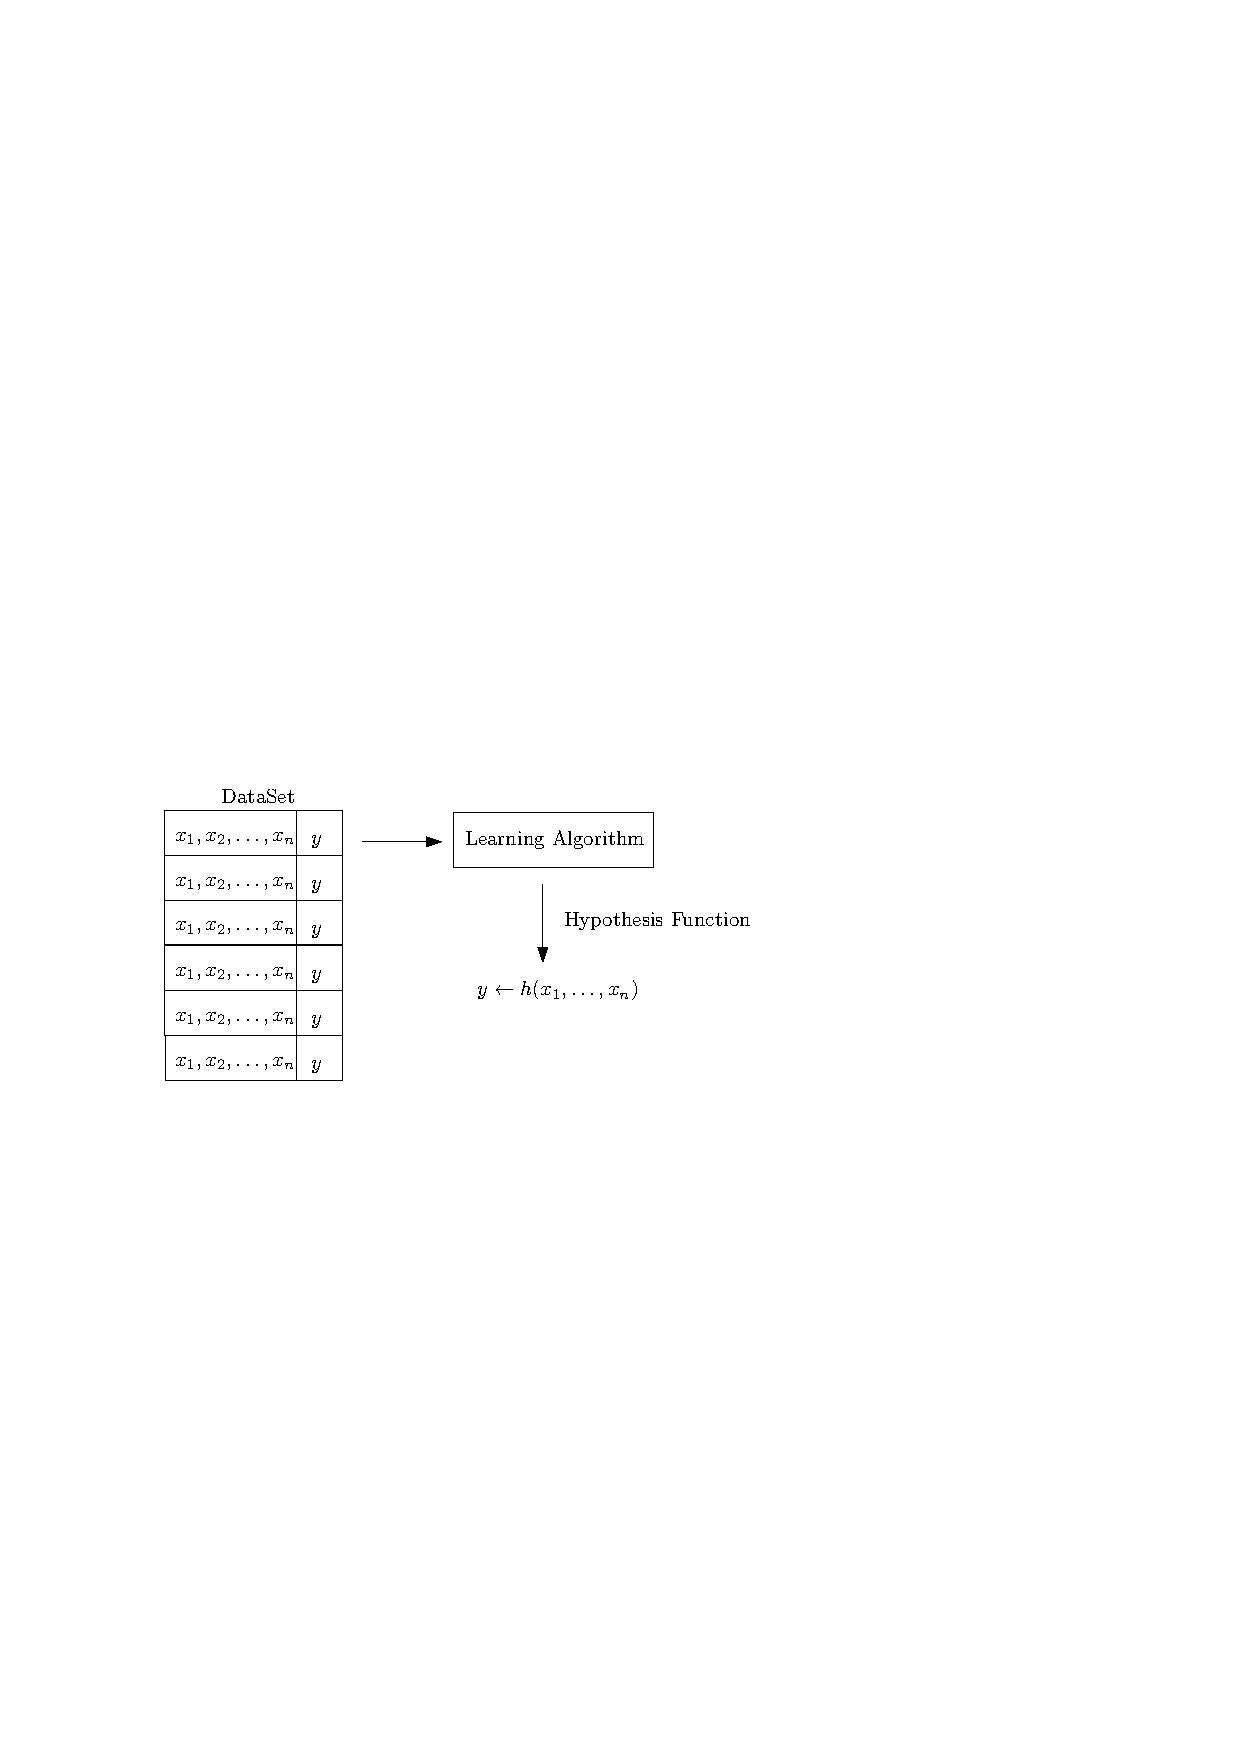
\includegraphics[scale=0.6]{pics/learning.pdf}
\end{figure}

} 
 
\end{frame}


\begin{frame}{Simple Linear Regression}
\scriptsize{
\begin{itemize}
 \item In simple linear regression, we have a single independent variable $x$ to model the dependent variable $\mathbf{y}$.

 \item The following linear relationship between the variables is assumed:

\begin{displaymath}
 y_i=\beta_{0}+\beta_{1}x_i +\epsilon_i \quad \forall i
\end{displaymath}

\item The parameter $\beta_{0}$ represents the intercept of the line (the value of $y$ when $x$ is zero).  

\item The parameter $\beta_{1}$ is the slope and represents the change of $\mathbf{y}$ when we vary the value of $\mathbf{x}$. The greater the magnitude of this parameter the greater the linear relationship between the variables.

\item The $\epsilon_{i}$ values correspond to the errors or \textbf{residuals} associated with the model.

\item We have to find a linear function or straight line $h_\beta$ that allows us to find an estimate of $y$, $\hat{y}$ for any value of $x$ with the minimum expected error.

\begin{displaymath}
h(x)=\beta_{0}+\beta_{1}x 
\end{displaymath}


\end{itemize}


} 
 
\end{frame}



\begin{frame}{Least Squares}
\scriptsize{
\begin{itemize}

 \item The ordinary least squares method is used to estimate  $\hat{\beta}_{0}$ and $\hat{\beta}_{1}$ by minimizing the sum of squared errors (SSE) of the observed data.

 \item Suppose we have $m$ observations of $\mathbf{y}$ and $\mathbf{x}$, we compute the sum of squared errors (SSE) or $E$ error as follows:

\begin{equation}
E = \sum_{i=1}^{m} (y_i-h(x_i))^2 =  \sum_{i=1}^{m} (y_i-\beta_{0}-\beta_{1}x_i)^2
\end{equation}

 \item To find the parameters that minimize the error we calculate the partial derivatives of SSE with respect to $\beta_{0}$ and $\beta_{1}$. Then we equal the derivatives to zero and solve the equation to find the parameter values.
 
 \begin{equation}
 \frac{\partial E}{ \partial \beta_0} = -2\sum_{i=1}^{m}(y_i-\beta_{0}-\beta_{1}x_i)=0
 \end{equation}

  \begin{equation}
 \frac{\partial E}{ \partial \beta_1} = -2\sum_{i=1}^{m}(y_i-\beta_{0}-\beta_{1}x)x_i=0
 \end{equation}



\end{itemize}



} 
\end{frame}

\begin{frame}{Least Squares (2)}
\scriptsize{
\begin{itemize}
 \item From the above system of equations the normal solutions are obtained:
  \begin{equation}
 \hat{\beta}_{1} = \frac{\sum_{i}^{m} (x_i-\overline{x})(y_i-\overline{y}) }{ \sum_{i}^{m} (x_i-\overline{x})^2}    
 \end{equation}

 \begin{equation}
 \hat{\beta}_{0} = \overline{y} -\beta_{1}\overline{x}    
 \end{equation}



\item The fitted model represents the line of least squared error.

\begin{figure}[h!]
	\centering
	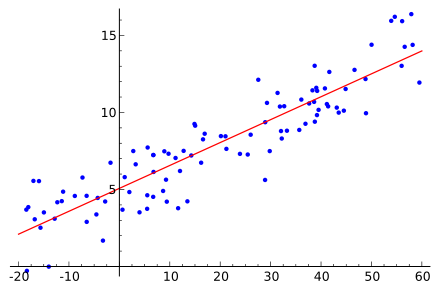
\includegraphics[scale=0.35]{pics/Linear_regression.png}
\end{figure}

\end{itemize}

} 
 
\end{frame}


\begin{frame}{Coefficient of Determination $R^2$}
\scriptsize{
\begin{itemize}
 \item  Once we have fitted our linear model we must evaluate the quality of the model.
 \item A very common metric is the coefficient of determination $R^2$. 
 \item  It is calculated from errors that are different than the SSE squared errors.
 \item The total sum squared error (SST)  is defined as the predictive error when we use the mean $\overline{y}$  to predict the response variable $y$ (it is very similar to the variance of the variable):
 \begin{displaymath}
  \text{SST} = \sum_{i}^{m}(y_i-\overline{y})^2  
 \end{displaymath}
 \item  Then we have the sum of squares explained by the model (SSM) which indicates the variability of the values predicted by the model with respect to the mean:
 \begin{displaymath}
  \text{SSM} = \sum_{i}^{m}(\hat{y}_i-\overline{y})^2 
 \end{displaymath}
  
\end{itemize}

}
\end{frame}

\begin{frame}{Coefficient of Determination $R^2$ (2)}
\scriptsize{
\begin{itemize}
 \item The coefficient of determination for a linear model $R^2$ is defined as:
 \begin{equation}
  R^2= \frac{\text{SSM}}{\text{SST}} = \frac{\sum_{i}^{m}(\hat{y}_i-\overline{y})^2 }{\sum_{i}^{m}(y_i-\overline{y})^2  }
 \end{equation}

 \item The coefficient takes values between $0$ to $1$ and the closer its value is to 1 the higher the quality of the model.
 
 \item The value of $R^2$ is equivalent to the linear correlation (Pearsons) between $y$ and $\hat{y}$ squared.
\begin{displaymath}
 R^2=\text{cor}(y,\hat{y})^2
\end{displaymath}
  
\end{itemize}


}
\end{frame}



\begin{frame}{Assumptions of the Linear Model}
\scriptsize{





Whenever we fit a linear model we are implicitly making certain assumptions about the data.  


\begin{block}{Assumptions}
\begin{enumerate}
\item Linearity: the response variable is linearly related to the attributes. 
\item  Normality: errors have zero mean normal distribution: $\epsilon_{i} \sim N(0,\sigma^2)$.
\item Homoscedasticity: errors have constant variance (same value $\sigma^2$).
\item Independence: errors are independent of each other.
 
\end{enumerate}
 
\end{block}

} 
\end{frame}


\begin{frame}{Probabilistic Interpretation}
\scriptsize{
\begin{itemize}
 \item Considering the above assumptions, we can see that the probability density (PDF) of the errors $\epsilon$ is defined by a normal of zero mean and constant variance:
 \begin{displaymath}
  \text{PDF}(\epsilon_{i})=\frac{1}{\sqrt{2\pi} \sigma} \exp \left(- \frac{\epsilon_{i}^{2}}{2\sigma^2}\right)
 \end{displaymath}
 \item This implies that:
  \begin{displaymath}
  \text{PDF}(y_i|x_{i};\beta)=\frac{1}{\sqrt{2\pi} \sigma} \exp \left(- \frac{(y_i - h_{\beta}(x_{i}) )^{2}}{2\sigma^2}\right)
 \end{displaymath}
\item Which implies that the distribution of $\mathbf{y}$ given the values of $\mathbf{x}$ and parameterized by $\beta$ follows a normal distribution.
 \item Then if one estimates the parameters of $\beta$ using maximum likelihood estimation one arrives at the same results as doing least squares estimation.
 \item This tells us that when we estimate the model parameters using least squares we are making the same probabilistic assumptions mentioned above.

\end{itemize}


}
 
\end{frame}


\begin{frame}{A signgicante test for $\beta$}
\scriptsize{
\begin{itemize}
 \item We can test if the value of $\beta$ is different from zero.

\end{itemize}


}
 
\end{frame}


\begin{frame}[fragile]{Example: a model of height}
\scriptsize{
\begin{itemize}
 \item  We are going to work with the dataset \verb+Howell1+ that has  partial census data for the Dobe area !Kung San, compiled from interviews conducted by Nancy Howell in the late 1960s. 
 \item The !Kung San are the most famous foraging population of the twentieth century, largely because of detailed quantitative studies by people like Howell.
 \end{itemize} 

 
 \begin{figure}[h!]
	\centering
	
\includegraphics[scale=0.6]{pics/San_Schmuck.jpg}
	\caption{By Staehler - Own work, CC BY-SA 4.0, \url{https://commons.wikimedia.org/w/index.php?curid=45076017}}
\end{figure}

 
}
\end{frame}


\begin{frame}[fragile]{Example: a model of height}
\scriptsize{
\begin{itemize}
 \item Each observation corresponds to an individual.
 \item The variables of the dataset are:
 \begin{enumerate}
 \scriptsize{
\item height: Height in cm
\item weight: Weight in kg
\item age: Age in years
\item male: Gender indicator
\item age.at.death: If deceased, age at death
\item alive: Indicator if still alive
  }
 \end{enumerate}
 
\item To see if it is worth doing a linear regression analysis, we look at the linear correlations between the variables

 \begin{verbatim}
> library(rethinking)
> data(Howell1)
> d <- Howell1
> cor(d)
          height    weight         age        male
height 1.0000000 0.9408222 0.683688567 0.139229021
weight 0.9408222 1.0000000 0.678335313 0.155442866
age    0.6836886 0.6783353 1.000000000 0.005887126
male   0.1392290 0.1554429 0.005887126 1.000000000
 \end{verbatim}

 
 
 
\end{itemize}
 
 
 
 
} 
\end{frame}


\begin{frame}[fragile]{Example: a model of height}
\scriptsize{
\begin{itemize}
 \item We can see that there is a significant positive correlation between \verb+Height+ and \verb+Age+.
 
 \item All we want for now are heights of adults in the sample. The reason to filter out nonadults for now is that height is strongly correlated with age, before adulthood. 
 
  \begin{verbatim}
   d2 <- d[ d$age >= 18 , ]
  \end{verbatim}

 \item Now age doesn't correlate with height:
 

  \begin{verbatim}
> cor(d2)
           height     weight         age       male
height  1.0000000  0.7547479 -0.10183776 0.69999340
weight  0.7547479  1.0000000 -0.17290430 0.52445271
age    -0.1018378 -0.1729043  1.00000000 0.02845498
male    0.6999934  0.5244527  0.02845498 1.00000000
  \end{verbatim} 
 
 
 \item Let's model height as a function of weight using a simple linear regression:
 \begin{displaymath}
  \text{height}(\text{weight})=\beta_0+\beta_1*\text{weight}
 \end{displaymath}
 
  \item In R the linear models are created with the command \verb+lm+ that receives as parameter a formula of the form \verb+y~x+ ($y=f(x)$).
 
 \begin{verbatim}
> reg1<-lm(Murder~Assault,USArrests)
> reg1

Call:
lm(formula = Murder ~ Assault, data = USArrests)

Coefficients:
(Intercept)      Assault  
    0.63168      0.04191    
 \end{verbatim}
 
 \item We can see that the coefficients of the model are $\beta_{0}=0.632$ and $\beta_{1}=0.042$. 
 
 


\end{itemize}
 
 
 
} 
\end{frame}

\begin{frame}[fragile]{Example: a model of height}
\scriptsize{
\begin{itemize}
 \item We can directly access the coefficients and store them in a variable:
 \begin{verbatim}
> reg1.coef<-reg1$coefficients
> reg1.coef
(Intercept)     Assault 
 0.63168266  0.04190863 
 \end{verbatim}
 
\item We can view various indicators about the linear model with the command \textbf{summary}:
 
\begin{verbatim}
> summary(reg1)
Residuals:
    Min      1Q  Median      3Q     Max 
-4.8528 -1.7456 -0.3979  1.3044  7.9256 

Coefficients:
            Estimate Std. Error t value Pr(>|t|)    
(Intercept) 0.631683   0.854776   0.739    0.464    
Assault     0.041909   0.004507   9.298  2.6e-12 ***
---
Signif. codes:  0 ‘***’ 0.001 ‘**’ 0.01 ‘*’ 0.05 ‘.’ 0.1 ‘ ’ 1

Residual standard error: 2.629 on 48 degrees of freedom
Multiple R-squared:  0.643,	Adjusted R-squared:  0.6356 
F-statistic: 86.45 on 1 and 48 DF,  p-value: 2.596e-12

\end{verbatim}
 
 \end{itemize}
 
 


} 
\end{frame}


\begin{frame}[fragile]{Example: a model of height}
\scriptsize{
\begin{itemize}
 \item We see that the coefficient of determination $R^2$ has a value of $0.643$ which is not so good but acceptable.
 
 
  \item We can conclude that the level of assaults while providing useful information to model a part of the variability of the homicide level is not enough to build a highly reliable model. 
  
  \item We can store the results of the command \verb+summary+ in a variable then access the coefficient of determination:
\begin{verbatim}
> sum.reg1<-summary(reg1)
> sum.reg1$r.squared
[1] 0.6430008   
\end{verbatim}

\item  We can also access the fitted values which are the values predicted by my model for the data used:
\begin{verbatim}
> reg1$fitted.values
       Alabama         Alaska        Arizona       Arkansas        
     10.522119      11.653652      12.952819       8.594322      
\end{verbatim}
 
 \end{itemize}
 

} 
\end{frame}



\begin{frame}[fragile]{Example: a model of height}
\scriptsize{
\begin{itemize}
 \item We can check that the squared linear correlation between my fitted and observed values for the response variable is equivalent to the coefficient of determination:
 
 \begin{verbatim}
> cor(Murder,reg1$fitted.values)^2
[1] 0.6430008
 \end{verbatim}

\item  Suppose now that we know the level of assault for two states in another period for two locations but I don't know the level of murders.

\item  We could use my linear model to predict the level of homicides.

\item To do this in R we must use the command \verb+predict.lm+ which receives the linear model and a data.frame with the new data:
\begin{verbatim}
> new.arrests<-data.frame(Assault=c(500,12))
> predict.lm(object=reg1,newdata=new.arrests)
        1         2 
21.585997  1.134586 
> # this is equivalent to:
> reg1.coef[1]+reg1.coef[2]*new.arrests
    Assault
1 21.585997
2  1.134586 
\end{verbatim}

 
 \end{itemize}
 

} 
\end{frame}


\begin{frame}{Multivariate Linear Regression}
\scriptsize{
\begin{itemize}
 \item Suppose we have $n$ independent variables:  $x_1,x_2,\dots,x_n$.
 \item Intuitively, these variables together could better explain the variability of the response variable $\mathbf{y}$ than a simple model.
 \item A multivariate linear model is defined as follows:
 \begin{displaymath}
 y_i=\beta_{0}+\beta_{1}x_{i,1}+ +\beta_{2}x_{i,2} + \cdots + \beta_{n}x_{i,n} +  \epsilon_i \quad \forall i \in \{1,m\}
\end{displaymath}
\item  In the multivariate model all the properties of the simple linear model are extended.

\item The problem can be represented in a matrix form:
\begin{displaymath}
 Y=X\beta+\epsilon
\end{displaymath}

\item Where $Y$ is a vector $m\times 1$ response variables:

\begin{displaymath}
 Y =
 \begin{pmatrix}
  y_{1} \\
  y_{2}  \\
  \vdots  \\
  y_{m}
 \end{pmatrix}
\end{displaymath}






\end{itemize}
 

}
\end{frame}

\begin{frame}{Multivariate Linear Regression (2)}
\scriptsize{
\begin{itemize} 
\item $X$ is a $m \times (n+1)$  matrix with the explanatory variables. We have $m$ observations of the $n$ variables.  The first column is constant equal to $1$ ($x_{i,0}=1 \quad \forall i$) to model the intercept variables $\beta_0$.

\begin{displaymath}
 X =
 \begin{pmatrix}
x_{1,0} &  x_{1,1} & x_{1,2} & \cdots & x_{1,n} \\
x_{2,0} &  x_{2,1} & x_{2,2} & \cdots & x_{2,n} \\
\vdots  &  \vdots  & \vdots  & \ddots & \vdots  \\
x_{m,0} &  x_{m,1} & x_{m,2} & \cdots & x_{m,n}
 \end{pmatrix}
\end{displaymath}

 \item Then, $\beta$ is a $(n+1) \times 1$ vector of parameters.

\begin{displaymath}
 \beta =
 \begin{pmatrix}
  \beta_{0}  \\
  \beta_{1}  \\
  \vdots    \\
  \beta_{n} 
 \end{pmatrix}
\end{displaymath}





\end{itemize}
 

}
\end{frame}

\begin{frame}{Multivariate Linear Regression (2)}
\scriptsize{
\begin{itemize}
\item Finally, $\epsilon$  is a $m \times 1$ vector with the model errors. 

\begin{displaymath}
 \epsilon =
 \begin{pmatrix}
  \epsilon_{1}  \\
  \epsilon_{2}  \\
  \vdots    \\
  \epsilon_{m} 
 \end{pmatrix}
\end{displaymath}

\item  Using matrix notation, we can see that the sum of squared errors (SSE) can be expressed as:
\begin{displaymath}
 \text{SSE} = (Y - X\beta)^{T}(Y-X\beta)
\end{displaymath}

\item Minimizing this expression by deriving the error as a function of $\beta$ and setting it equal to zero leads to the normal equations:

\begin{displaymath}
   \hat{\beta} = (X^{T}X)^{-1} X^{T}Y
\end{displaymath}


\end{itemize}


}

\end{frame}





\begin{frame}[fragile]{Linear Regression in R}
\scriptsize{
\begin{itemize}
 \item  Now we will study a multiple linear regression.
 \item We can see that the variable \textbf{Rape} representing the level of rapes has a lower correlation with the number of assaults and with the number of homicides than the correlation that these two variables have with each other.
 \item  Let's fit the following linear multi-variate model:
 \begin{displaymath}
 \text{Rape}=\beta_{0}+\beta_{1}*\text{Assault}+\beta_{2}*\text{Murder}
 \end{displaymath}
 \item In R to add more variables to the linear model we add them with the operator \textbf{+} :
\begin{verbatim}
reg2<-lm(Rape~Assault+Murder,USArrests)
\end{verbatim}



 
 \end{itemize}
 

} 
\end{frame}


\begin{frame}[fragile]{Linear Regression in R (7)}
\scriptsize{

\begin{verbatim}
> summary(reg2)

Residuals:
    Min      1Q  Median      3Q     Max 
-17.243  -3.171  -1.171   3.281  18.511 

Coefficients:
            Estimate Std. Error t value Pr(>|t|)    
(Intercept)  8.35011    2.32912   3.585 0.000799 ***
Assault      0.06716    0.02044   3.286 0.001927 ** 
Murder       0.18155    0.39108   0.464 0.644619    
---
Signif. codes:  0 ‘***’ 0.001 ‘**’ 0.01 ‘*’ 0.05 ‘.’ 0.1 ‘ ’ 1

Residual standard error: 7.124 on 47 degrees of freedom
Multiple R-squared:  0.4451,	Adjusted R-squared:  0.4215 
F-statistic: 18.85 on 2 and 47 DF,  p-value: 9.755e-07

\end{verbatim}

\begin{itemize}
\item In this case the coefficient of determination is low. So we will have low confidence in the quality of the model.
 \end{itemize}
 

} 
\end{frame}

\begin{frame}[fragile]{Linear Regression in R (8)}
\scriptsize{
\begin{itemize}
 \item When we had a simple regression we could see the fitted model as a line.
 \item Now that we have two independent variables we can see the fitted model as a plane.
 \item If we had more independent variables our model would be a hyper-plane.
 \item We can plot the plane of our linear model of two independent variables and one dependent variable in R as follows:
 \end{itemize}

\begin{verbatim}
library("scatterplot3d")
s3d <- scatterplot3d(USArrests[,c("Assault","Murder","Rape")],
                     type="h", highlight.3d=TRUE,
                     angle=55, scale.y=0.7, pch=16, 
                     main="Rape~Murder+Rape")
s3d$plane3d(reg2, lty.box = "solid")

\end{verbatim}




} 
\end{frame}

\begin{frame}{Linear Regression in R (9)}
 
\begin{figure}[h!]
	\centering
	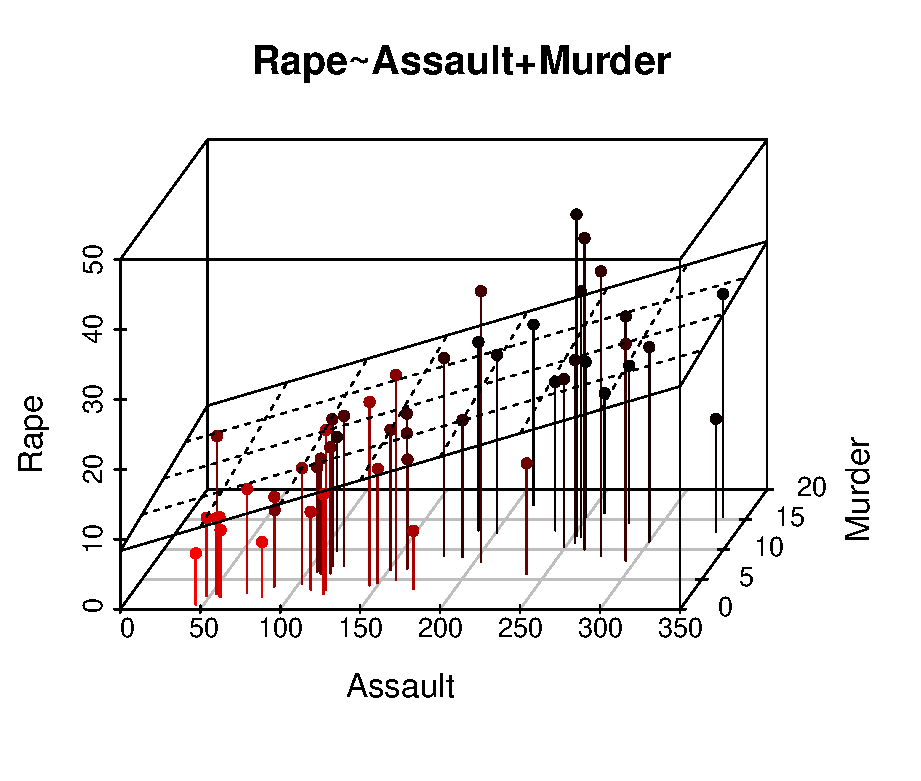
\includegraphics[scale=0.6]{pics/reg3d.pdf}
\end{figure}
 
\end{frame}



\begin{frame}{Bonus: Four Cardinal Rules of Statistics by Daniela Witten}
\scriptsize{

Now that we have concluded the chapter on Frequentist inference, it is good to discuss the points discussed by Daniela Witten on a tweet.

\begin{figure}[h!]
	\centering
	
\includegraphics[scale=0.3]{pics/witten.png}
\end{figure}


\begin{block}{One: Correlation does not imply causation}
\begin{itemize}
 \item Yes, I know you know this, but it’s so easy to forget! Yeah, YOU OVER THERE, you with the p-value of 0.0000001 — yes, YOU!! That’s not causation.
 \item No matter how small the p-value for a regression of IQ onto shoe size is, that doesn’t mean that big feet cause smarts!!  It just means that grown-ups tend to have bigger feet and higher IQs than kids.
 \item So, unless you can design your study to uncover causation (very hard to do in most practical settings — the field of causal inference is devoted to understanding the settings in which it is possible), the best you can do is to discover correlations.  Sad but true.
\end{itemize}

 
\end{block}




} 
\end{frame}

\begin{frame}{Bonus: Four Cardinal Rules of Statistics by Daniela Witten}
\scriptsize{


\begin{block}{Two:  a p-value is just a test of sample size}
\begin{itemize}
 \item  Read that again — I mean what I said!  If your null hypothesis doesn't hold (and null hypotheses never hold IRL) then the larger your sample size, the smaller your p-value will tend to be.
 \item If you’re testing whether mean=0 and actually the truth is that mean=0.000000001, and if you have a large enough sample size, then YOU WILL GET A TINY P-VALUE.
 \item Why does this matter? In many contemporary settings (think: the internet), sample sizes are so huge that we can get TINY p-values even when the deviation from the null hypothesis is negligible. In other words, we can have STATISTICAL significance w/o PRACTICAL significance.
 \item Often, people focus on that tiny p-value, and the fact that the effect is of **literally no practical relevance** is totally lost.
 \item This also means that with a large enough sample size we can reject basically ANY null hypothesis (since the null hypothesis never exactly holds IRL, but it might be “close enough” that the violation of the null hypothesis is not important). 
 \item Want to write a paper saying Lucky Charms consumption is correlated w/blood type? W/a large enough sample size, you can get a small p-value.  (Provided there’s some super convoluted mechanism with some teeny effect size… which there probably is, b/c IRL null never holds)
\end{itemize}

 
\end{block}


} 
\end{frame}



\begin{frame}{Bonus: Four Cardinal Rules of Statistics by Daniela Witten}
\scriptsize{


\begin{block}{Three: seek and you shall find}
\begin{itemize}
 \item If you look at your data for long enough, you will find something interesting, even if only by chance! 
 \item  In principle, we know that we need to perform a correction for multiple testing if we conduct a bunch of tests.
\item But in practice, what if we decide what test(s) to conduct AFTER we look at data?  Our p-value will be misleadingly small because we peeked at the data.  Pre-specifying our analysis plan in advance keeps us honest… but in reality, it’s hard to do!!!
\end{itemize}

 
\end{block}


\begin{itemize}
\item Everyone is asking me about the mysterious and much-anticipated fourth rule of statistics. The answer is simple: we haven’t figured it out yet.... that’s the reason we need to do research in statistics
\end{itemize}

} 
\end{frame}

%%%%%%%%%%%%%%%%%%%%%%%%%%%
%%%%%%%%%%%%%%%%%%%%%%%%%%%
\begin{frame}[allowframebreaks]\scriptsize
\frametitle{References}
\bibliography{bio}
\bibliographystyle{apalike}
%\bibliographystyle{flexbib}
\end{frame}  





%%%%%%%%%%%%%%%%%%%%%%%%%%%

\end{document}
